\section{Análise Teórica e Projeto do Filtro}

O projeto do filtro ativo passa-baixa Butterworth de $4^{\text{a}}$ ordem segue uma metodologia estruturada em três etapas analíticas fundamentais: a definição matemática do filtro-protótipo normalizado, a dedução algébrica de sua função de transferência baseada na topologia escolhida e, finalmente, a aplicação dos fatores de escalonamento de magnitude e frequência \cite{nilsson}.

\subsection{Topologia do Circuito e Modelo do Amplificador Operacional}

A implementação física de filtros ativos de ordem superior ($n \ge 2$) é tipicamente realizada pelo cascateamento de estágios de segunda ordem. Para o presente projeto, adotou-se a clássica topologia \textit{Sallen-Key}. É imperativo destacar a dualidade topológica desta configuração: enquanto em um filtro passa-alta os capacitores encontram-se em série com o sinal de entrada e os resistores em derivação para o terra \cite{nilsson}, o filtro passa-baixa objeto deste estudo inverte rigorosamente essa disposição. No filtro passa-baixa, os elementos resistivos ($R_1, R_2$) formam o caminho série de condução do sinal, enquanto os elementos capacitivos ($C_1, C_2$) assumem as posições de derivação e realimentação[cite: 731, 732, 733, 734, 735, 736, 737].

\begin{figure}[htbp]
	\centering
	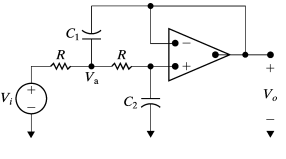
\includegraphics[width=0.7\textwidth]{FIGURAS/esquematico_filtro_passabaixa_ativo_butterworth.png}
	\caption{Topologia Sallen-Key para um estágio passa-baixa ativo de segunda ordem.}
	\label{fig:topologia_sallenkey_pb}
\end{figure}

A análise do circuito repousa sobre as propriedades do Amplificador Operacional (AmpOp) ideal. Assume-se que o ganho diferencial em malha aberta tende ao infinito ($A \rightarrow \infty$)[cite: 721]. Consequentemente, para que a tensão de saída $V_o$ seja finita, a diferença de potencial entre as entradas inversora e não-inversora deve ser nula ($V^+ - V^- = 0$)[cite: 728]. Além disso, a impedância de entrada infinita garante que não há fluxo de corrente adentrando os terminais do AmpOp ($I^+ = I^- = 0$)[cite: 728].

\begin{figure}[htbp]
	\centering
	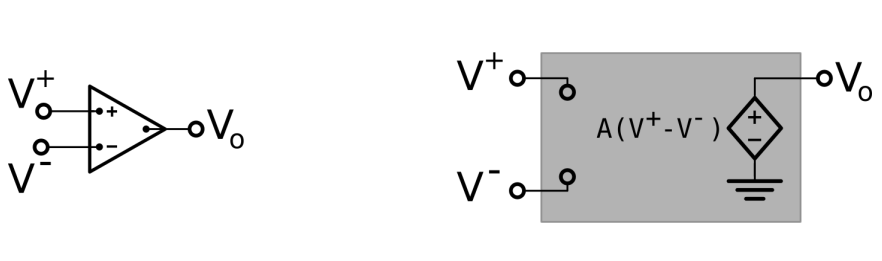
\includegraphics[width=0.5\textwidth]{FIGURAS/modelo_ampop.png}
	\caption{Modelo equivalente do amplificador operacional ideal com ganho $A \rightarrow \infty$.}
	\label{fig:modelo_ampop}
\end{figure}

Como o amplificador está configurado como um seguidor de tensão (realimentação negativa direta da saída para a entrada inversora), estabelece-se a restrição de que $V_o = V^- = V^+$.

\subsection{Dedução da Função de Transferência do Protótipo}

Considerando o circuito referenciado na seção "Prólogo" do roteiro [cite: 729], que dita a estrutura básica para cada módulo de duplo polo[cite: 730], aplica-se a Lei de Kirchhoff das Correntes (LKC) no nó intermediário $V_a$ e no nó não-inversor $V^+$ no domínio da frequência complexa de Laplace ($s$). 

Para simplificar a síntese, adota-se resistores de valores iguais ($R_1 = R_2 = R$).
A equação nodal para o nó $V^+$ é:
\begin{equation}
	\frac{V^+ - V_a}{R} + V^+ (sC_2) = 0 \implies V_a = V_o(1 + sRC_2)
\end{equation}

A equação nodal para o nó $V_a$ é:
\begin{equation}
	\frac{V_a - V_i}{R} + \frac{V_a - V^+}{R} + (V_a - V_o)(sC_1) = 0
\end{equation}

Substituindo $V_a$ na equação acima e manipulando algebricamente, obtém-se a função de transferência canônica $H(s) = \frac{V_o(s)}{V_i(s)}$ para um estágio Sallen-Key passa-baixa:
\begin{equation}
	H(s) = \frac{1}{s^2 (R^2 C_1 C_2) + s(2RC_2) + 1}
\end{equation}

\subsection{Aproximação de Butterworth e Síntese de 4ª Ordem}

O projeto especifica uma resposta de Butterworth, conhecida por apresentar uma banda de passagem maximamente plana \cite{nilsson}. Os polinômios de Butterworth são normalizados ajustando a frequência de corte para $\omega_c = 1\text{ rad/s}$[cite: 901]. Para um filtro de $4^{\text{a}}$ ordem ($n=4$), o polinômio correspondente $B_4(s)$ possui raízes conjugadas que resultam na seguinte fatoração quadrática[cite: 914, 919]:
\begin{equation}
	B_4(s) = (s^2 + 0.765367s + 1)(s^2 + 1.847759s + 1)
\end{equation}

Logo, o filtro completo requer o cascateamento de dois estágios Sallen-Key independentes, de modo que $H_{total}(s) = H_1(s) \cdot H_2(s)$. 
Igualando o denominador da equação teórica deduzida à forma genérica do protótipo $s^2 + bs + 1$[cite: 756], estabelecem-se as seguintes condições analíticas:
\begin{align}
	R^2 C_1 C_2 &= 1 \\
	2 R C_2 &= b \implies C_2 = \frac{b}{2R} \quad \text{e} \quad C_1 = \frac{2}{Rb}
\end{align}

Para o \textbf{filtro-protótipo normalizado}, adota-se $R = 1\ \Omega$ e $\omega_c = 1\text{ rad/s}$[cite: 928]. Extraem-se assim as capacitâncias de protótipo para cada estágio:
\begin{itemize}
	\item \textbf{Estágio 1 ($b_1 = 0.765367$):} $C_{1a} = 2.6131\text{ F}$ e $C_{2a} = 0.3827\text{ F}$.
	\item \textbf{Estágio 2 ($b_2 = 1.847759$):} $C_{1b} = 1.0824\text{ F}$ e $C_{2b} = 0.9239\text{ F}$.
\end{itemize}

\subsection{Escalonamento de Frequência e Magnitude}

Para traduzir o modelo ideal em um circuito construível, realiza-se a mudança de escala bidimensional[cite: 929, 930]. O fator de escalonamento de frequência ($k_f$) desloca a frequência de corte de $1\text{ rad/s}$ para a frequência alvo de projeto, $f_c = 50\text{ Hz}$[cite: 742]:
\begin{equation}
	k_f = \omega_c = 2\pi(50) = 314.16\text{ rad/s}
\end{equation}

O fator de escalonamento de amplitude ($k_a$) altera as impedâncias internas sem modificar a resposta em frequência[cite: 931, 943]. Como requisito estrito do projeto, os capacitores práticos não devem exceder $100\text{ nF}$[cite: 770]. As transformações aplicadas obedecem as seguintes premissas matemáticas[cite: 945]:
\begin{equation}
	R_{real} = k_a R \quad \text{e} \quad C_{real} = \frac{C}{k_a k_f}
\end{equation}

\begin{figure}[htbp]
	\centering
	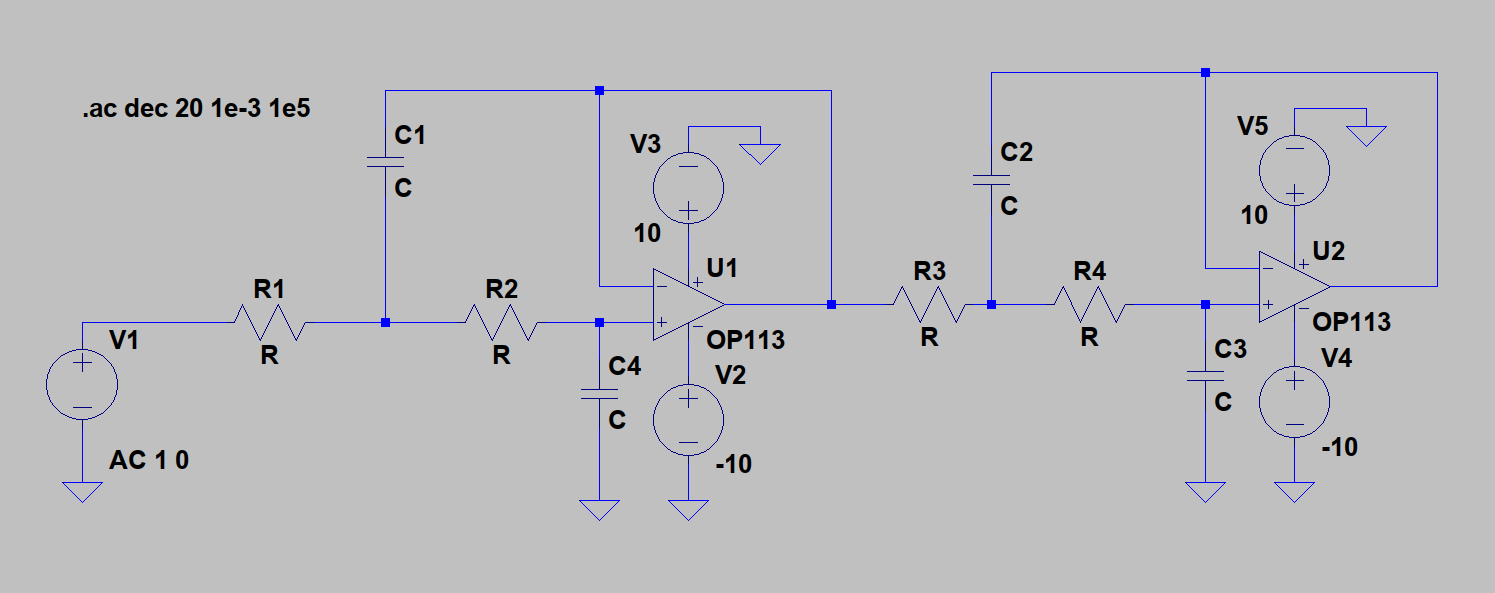
\includegraphics[width=0.9\textwidth]{FIGURAS/esquematico_sallenkey_completo_ltspice.png}
	\caption{Simulação esquemática da topologia de filtro ativo Sallen-Key completa montada para o projeto.}
	\label{fig:ltspice_esquematico_completo}
\end{figure}

A partir do escalonamento, os componentes são recalculados e aproximados para os valores comerciais da série E24 para viabilizar a implementação física no laboratório e a simulação computacional via \textit{LTSpice} \cite{ltspice}.